\documentclass[10pt]{beamer}
\usepackage{inputenc}
\usepackage{graphicx}
\usepackage{enumerate}
\usepackage{listings}
\usepackage{caption, subcaption}
\captionsetup[subfigure]{justification=centering}
\captionsetup{font=scriptsize,labelfont=scriptsize}
\usepackage{amsmath}
\usepackage{amssymb}
\usepackage{amsthm}
\usetheme{metropolis}    
\usepackage{verbatim}
\usepackage{alltt}
\usepackage{xcolor}
\usepackage{appendixnumberbeamer}
\usepackage{animate}
\usepackage{xmpmulti}
\usepackage{threeparttable, longtable}
\usepackage{booktabs}
\usepackage{setspace}
\usepackage{adjustbox}
\usepackage[T1]{fontenc}
\usepackage[colorlinks=true, allcolors=blue]{hyperref}
% \usepackage{color,soul}
\usepackage{tikz}
\usepackage{multirow}
\usepackage{float}
\usepackage{placeins}

\usepackage{tikz}
\usetikzlibrary{tikzmark,overlay-beamer-styles, calc}

\def\signed #1{{\leavevmode\unskip\nobreak\hfil\penalty50\hskip1em
		\hbox{}\nobreak\hfill #1%
		\parfillskip=0pt \finalhyphendemerits=0 \endgraf}}

\newsavebox\mybox
\newenvironment{aquote}[1]
{\savebox\mybox{#1}\begin{quote}\openautoquote\hspace*{-.7ex}}
	{\unskip\closeautoquote\vspace*{1mm}\signed{\usebox\mybox}\end{quote}}
\newcommand{\backupbegin}{
	\newcounter{finalframe}
	\setcounter{finalframe}{\value{framenumber}}
}
\newcommand{\backupend}{
	\setcounter{framenumber}{\value{finalframe}}
}
\usepackage[normalem]{ulem}
\useunder{\uline}{\ul}{}
\makeatletter
\setbeamertemplate{footline}
{
	\leavevmode%
	\hbox{%
		\begin{beamercolorbox}[wd=.15\paperwidth,ht=2.25ex,dp=1ex,center]{institute in head/foot}%
			\usebeamerfont{title in head/foot}%
			%  \insertshortauthor 
		\end{beamercolorbox}%
		\begin{beamercolorbox}[wd=.6\paperwidth,ht=2.25ex,dp=1ex,center]{institute in head/foot}%
			\usebeamerfont{title in head/foot}%
			\insertshorttitle
		\end{beamercolorbox}%
		\begin{beamercolorbox}[wd=.15\paperwidth,ht=2.25ex,dp=1ex,center]{institute in head/foot}%
			\usebeamerfont{title in head/foot}%
			\insertshortdate
		\end{beamercolorbox}%
		\begin{beamercolorbox}[wd=.1\paperwidth,ht=2.25ex,dp=1ex,right]{institute in head/foot}%
			\usebeamerfont{title in head/foot} 
			% \insertframenumber{} / \inserttotalframenumber\hspace*{2ex} 
                \insertframenumber{} \hspace*{2ex} 
	\end{beamercolorbox}}%
}

\definecolor{blueucl}{RGB}{0,87,156} 
\setbeamercolor{itemize item}{fg = blueucl}
\setbeamercolor{itemize subitem}{fg = blueucl}
\setbeamercolor{enumerate item}{fg = blueucl}
\setbeamercolor{enumerate subitem}{fg = blueucl}
\setbeamertemplate{itemize item}[triangle]
\setbeamercolor{progress bar}{fg=blueucl}
\setbeamercolor{alerted text}{fg = blueucl}

\lstset{numbers=left, numberstyle=\tiny, stepnumber=1,firstnumber=1,
	numbersep=5pt,
	stringstyle=\ttfamily,
	basicstyle=\footnotesize, 
	showstringspaces=false, 
	stringstyle=\color{blueucl}, 
	tabsize=1
}
\makeatother
\setbeamertemplate{caption}[numbered]
\newcommand{\ep}{\varepsilon}
\newtheorem{assumption}{Assumption}
\newtheorem{proposition}{Proposition}

\title[FlowTrading]{Flow Trading Format: A Laboratory Test}
\author[DF-YL-KL]{Dan Friedman, Yilin Li, Kristian L\'opez Vargas (UCSC)}
\institute[UCSC]{}  

\date[4/27/2024]{\vspace{1cm} \textbf{BABEEW - UC DAVIS} \\
April 27, 2024}

\begin{document}
\maketitle

% \tableofcontents

%%%%%%%%%%%%%%%%%%%%%%%%%%%%%%%%%%%%%%
\section{Motivation}
\begin{frame}{
The continuous double auction (CDA) market format}
\begin{itemize}
\item dominated in 20th century financial markets 
\item but design is now problematic.  %\pause
\end{itemize}
Problems arise from:
\begin{itemize}
\item strict price/time priority and 
\item a coarse price grid, 
\item unequal access to computing and telecom tech.

\end{itemize} %\pause
The result is a ``tilted playing field'': 
% huge investment to acquire millisecond advantage to snap up stale bids/asks, causing
%\pause
\begin{enumerate}
\item HFTs' perverse incentives impact slower traders
\item Unequal possibilities to prevent price impact
% \item unequal access: ``tilted playing field''
% \item 10's or 100's of \$billions in unproductive rent-seeking, %\pause
% \item reduced true liquidity due to toxic takers %\pause
% \item increased danger of ``flash crashes,'' as algorithms interact.
   \end{enumerate}
\end{frame}

\begin{frame}{Reform proposals}
Proposed design of financial markets include:
    \begin{itemize}
\item IEX: see e.g., M. Lewis (2014), Aldrich and Friedman (2023); %\pause
\item FBA: see e.g., Budish et al (2015), Aldrich and Lopez Vargas (2019); and %\pause
\item Flow markets:  Kyle \& Lee (2017), Budish et al. (2023).
\end{itemize}
% The last is my personal favorite, and the subject of today's presentation.
\end{frame}

% \begin{frame}{Claimed Benefits of Flow markets.}
% Its proponents argue that Flow markets provide a
% \begin{enumerate}
%  \item natural solution to HFT problems, and a %\pause
% \item natural way to minimize price impact. 
% \begin{itemize}
%     \item CDA provokes arms race to shred orders. 
% \end{itemize} %\pause
% \item The format also facilitates combinatorial trade for inter-related assets (`package trades').
% \end{enumerate} 
% \end{frame}

\begin{frame}{Our project}

Our paper \textbf{compares CDA and Flow} market formats in a ``simple'' lab environment (finitely divisible units / induced supply - demand are for a \textbf{large set of units}). 
%\pause

This environment is \textbf{not} designed to study HFTs' incentives. \\ %\pause 
It highlights the basic functioning of the two formats, and how traders deal with price impact. %\pause 

We compare:
\begin{itemize}
\item traders' behavior %\pause
\item price stability %\pause
\item trading volume, and %\pause
\item informational and allocative efficiency. 
\end{itemize} 

Sets stage for (but does not yet include) investigation of package bidding.

\end{frame}

\section{Market Formats}

% \begin{frame}{CDA Example Market}
\begin{frame}{Market Format 1: CDA - Example}
    \begin{figure}[H]
        \centering
        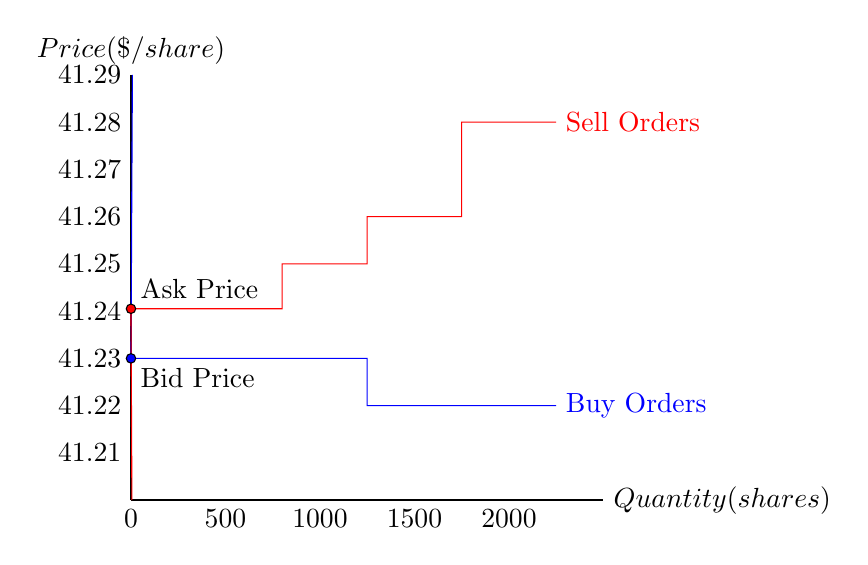
\begin{tikzpicture}[scale=.6]
        \draw[thick,-] (0,0) -- (0,9) node[above]{$Price (\$/share)$};
        \draw[thick,-] (0,0)--(10,0) node[right]{$Quantity (shares)$};
        \node[left] at (0,1) {$41.21$};
        \node[left] at (0,2) {$41.22$};
        \node[left] at (0,3) {$41.23$};
        \node[left] at (0,4) {$41.24$};
        \node[left] at (0,5) {$41.25$};
        \node[left] at (0,6) {$41.26$};
        \node[left] at (0,7) {$41.27$};
        \node[left] at (0,8) {$41.28$};
        \node[left] at (0,9) {$41.29$};
        \node[below] at (2,0) {$500$};
        \node[below] at (4,0) {$1000$};
        \node[below] at (6,0) {$1500$};
        \node[below] at (8,0) {$2000$};
        \node[below] at (0,0) {$0$};
        \draw[blue,solid] (0.03,9) -- (0,3) -- (2,3) -- (2,3) -- (5,3) -- (5,2) -- (9,2) node[right]{Buy Orders} ;
        \draw[red,solid] (0.02,0) -- (0,4.05) -- (3.2,4.05) -- (3.2,5) -- (5,5) -- (5,6) -- (7,6) -- (7,8) -- (9,8) node[right]{Sell Orders};
        \node[above right] at (0,4.05) {Ask Price};
        \draw[fill=red] (0,4.05) circle [radius=.1];
        \node[below right] at (0,3) {Bid Price};
        \draw[fill=blue] (0,3) circle [radius=.1];
        \end{tikzpicture}
        \caption{Standard Limit Order Book}
    \end{figure}
\end{frame}


\begin{frame}{Market Format 1: CDA - Example (at one instant)}
    \begin{figure}[H]
        \centering
        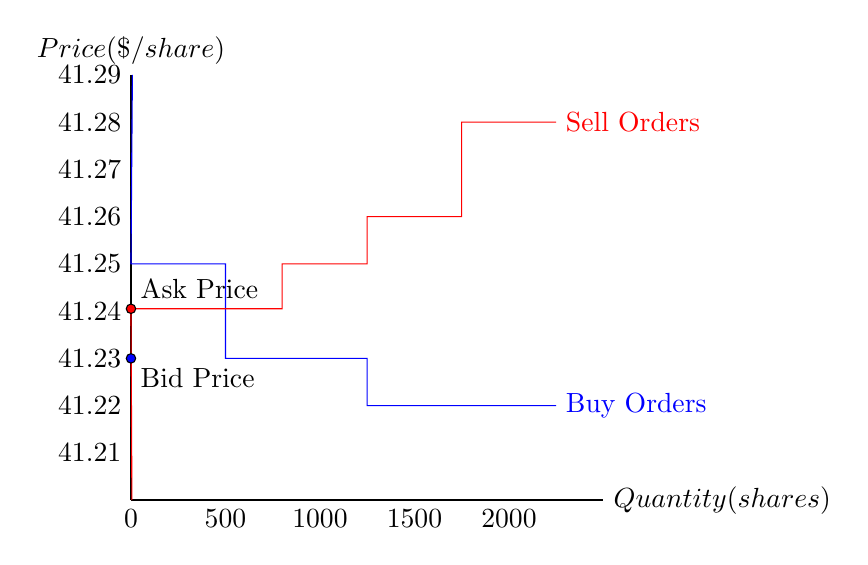
\begin{tikzpicture}[scale=.6]
        \draw[thick,-] (0,0) -- (0,9) node[above]{$Price (\$/share)$};
        \draw[thick,-] (0,0)--(10,0) node[right]{$Quantity (shares)$};
        \node[left] at (0,1) {$41.21$};
        \node[left] at (0,2) {$41.22$};
        \node[left] at (0,3) {$41.23$};
        \node[left] at (0,4) {$41.24$};
        \node[left] at (0,5) {$41.25$};
        \node[left] at (0,6) {$41.26$};
        \node[left] at (0,7) {$41.27$};
        \node[left] at (0,8) {$41.28$};
        \node[left] at (0,9) {$41.29$};
        \node[below] at (2,0) {$500$};
        \node[below] at (4,0) {$1000$};
        \node[below] at (6,0) {$1500$};
        \node[below] at (8,0) {$2000$};
        \node[below] at (0,0) {$0$};
        \draw[blue,solid] (0.03,9) -- (0,5) -- (2,5) -- (2,3) -- (5,3) -- (5,2) -- (9,2) node[right]{Buy Orders} ;
        \draw[red,solid] (0.02,0) -- (0,4.05) -- (3.2,4.05) -- (3.2,5) -- (5,5) -- (5,6) -- (7,6) -- (7,8) -- (9,8) node[right]{Sell Orders};
        \node[above right] at (0,4.05) {Ask Price};
        \draw[fill=red] (0,4.05) circle [radius=.1];
        \node[below right] at (0,3) {Bid Price};
        \draw[fill=blue] (0,3) circle [radius=.1];
        \end{tikzpicture}
        \caption{Standard Limit Order Book}
    \end{figure}
\end{frame}



\begin{frame}{Market Format 2: FLOW - Example - Individual}
    \begin{figure}
        \centering
        
\includegraphics[width=\textwidth]{figures/flow.png}
        \caption{Continuous Scaled Limit Orders}
        \label{fig:flow}
    \end{figure}
\end{frame}

\begin{frame}{Market Format 2: The FLOW}
    \begin{itemize}
\item Continuous scaled limit orders have \textbf{five parameters}: $\rightarrow$ ``\underline{Buy/Sell} up to a cumulative total of  \underline{$Q_{max}$} (shares) at maximum rate \underline{$U_{max}$} (shares per hour) at prices between \underline{$P_{L}$} and \underline{$P_{H}$} (dollars per share)."
\item Consider a buy order. The (buying rate or) flow demand $U(p(t))$ is the decreasing pw linear function:
\begin{align}
                U{(p(t))}=
                \begin{cases}
                    U_{max} & \text{ if } p{(t)} < P_{L} \\
                    (\frac{P_{H}-p(t)}{P_{H}-P_{L}})U_{max} & \text{ if } P_L \leq p{(t)} \leq P_H \\
                    0  & \text{ if } p{(t)} > P_{H} \\
                \end{cases}
\end{align}
        where $p(t)$ is the clearing price at time $t$.
\item The flow supply (rate) is an analogous pw linear monotone \textbf{increasing} function of $p(t)$
    \end{itemize}
\end{frame}

\begin{frame}{Market Format 2: FLOW - Example - Market}
    \begin{figure}[H]
        \centering
        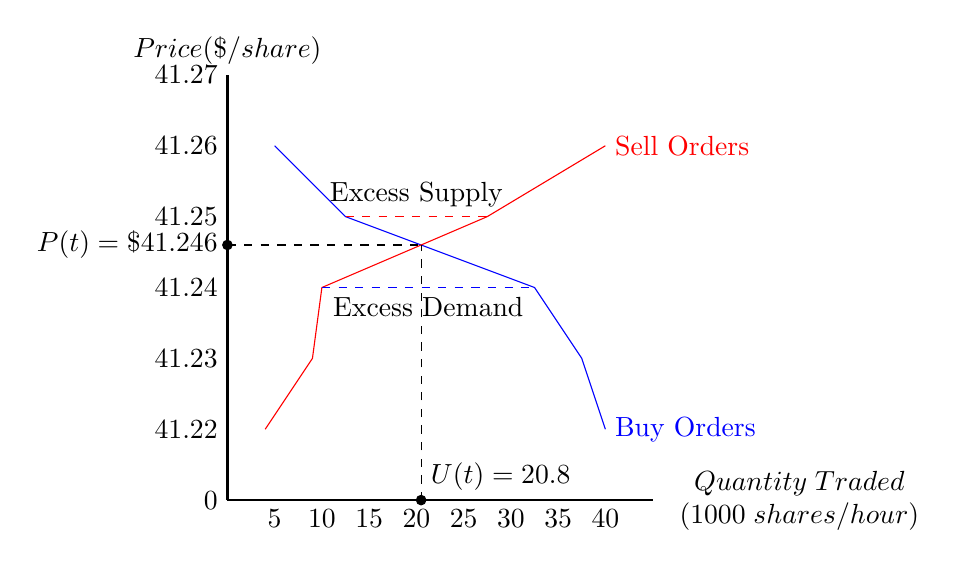
\begin{tikzpicture}[scale=0.6]
            \draw[thick,-] (0,0) -- (0,9) node[above]{$Price (\$/share)$};
            \draw[thick,-] (0,0)--(9,0) node[right]{\begin{tabular}{c}
                 $Quantity \; Traded$ \\
                 $(1000 \; shares/hour)$
            \end{tabular}};
            \node[left] at (0,1.5) {$41.22$};
            \node[left] at (0,3.0) {$41.23$};
            \node[left] at (0,4.5) {$41.24$};
            \node[left] at (0,6.0) {$41.25$};
            \node[left] at (0,7.5) {$41.26$};
            \node[left] at (0,9.0) {$41.27$};
            \node[below] at (1,0) {$5$};
            \node[below] at (2,0) {$10$};
            \node[below] at (3,0) {$15$};
            \node[below] at (4,0) {$20$};
            \node[below] at (5,0) {$25$};
            \node[below] at (6,0) {$30$};
            \node[below] at (7,0) {$35$};
            \node[below] at (8,0) {$40$};
            \node[left] at (0,0) {$0$};
            \draw[blue,solid] (1,7.5) -- (2.5,6.0) -- (6.5,4.5) -- (7.5,3) -- (8,1.5) node[right]{Buy Orders} ;
            \draw[red,solid] (0.8,1.5) -- (1.8,3) -- (2,4.5) -- (5.5,6) -- (8,7.5) node[right]{Sell Orders};
            \draw[red,dashed] (2.5,6.0) -- (5.5,6.0);
            \draw[blue,dashed] (2,4.5) -- (6.5,4.5);
            \node[black,above] at (4,6.0) {Excess Supply};
            \node[black,below] at (4.25,4.5) {Excess Demand};
            \draw[dashed] (4.1,0) -- (4.1,5.4);
            \draw[dashed] (0,5.4) -- (4.1,5.4);
            \node[above right] at (4.1,0) {$U(t)=20.8$};
            \draw[fill] (4.1,0) circle [radius=.1];
            \node[left] at (0,5.4) {$P(t)=\$41.246$};
            \draw[fill] (0,5.4) circle [radius=.1];
        \end{tikzpicture}
        \caption{Continuous Scaled Limit Order Book}
    \end{figure}
\end{frame}

\begin{frame}{Market Format 2: FLOW}
\begin{itemize}
\item Both the downward sloping demand schedule and upward sloping supply schedule are \textbf{piece-wise linear} functions of price $\rightarrow$ \textbf{unique} price and rate of shares per hour. %\pause
\item All continuous scaled limit orders ares treated \textbf{symmetrically} and executed \textbf{simultaneously} at the market clearing price %\pause
        \item \textbf{opportunities} to do order \textbf{shredding} are now \textbf{distributed equally} across agents, as now instructions to shred are \textbf{``moved into the exchange''} %\pause
        \item Consequently, now the
        \textbf{fastest trader} or the ones that can send massive numbers of messages to update orders are not rewarded
    \end{itemize}
\end{frame}

\section{Lab Implementation}

\begin{frame}{Experiment Design: Main Elements}
    \begin{itemize}
        \item Markets of \textbf{8} traders, 22 trading periods of two minutes (2 practice + \textbf{20 paid periods})
        \item \textbf{Incentives to trade}: In each trading period, the computer provides a \textbf{buy or sell contract} committing to buy or sell up to $x$ shares at some point during the trading period (e.g., Computer will buy up to 300 shares from you at price 13 ECU at second 115) 
        \item Contracts are private information %\pause
        % \item Subjects' inventories are restricted to be $[-Q_{contract}, 0]$ for those with a sell contract or $[0, Q_{contract}]$ for those with a buy contract
        \item \textbf{Choice Space}: Subjects can submit or update buy and/or sell orders at any time. %\pause
        \item \textbf{Treatments}: \{CDA, FLOW\} (between-group)
        \item Three sets of contracts varied across 5 blocks of 4 periods each. 
    \end{itemize}
\end{frame}

\begin{frame}{Experiment Design: Contracts}
    
\begin{figure}
    \centering
    % \caption{Contract Configurations}
    \begin{subfigure}[c]{0.33\linewidth}
        \centering
            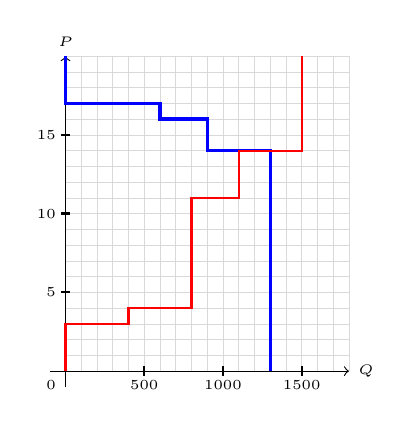
\begin{tikzpicture}[scale=.2]
                % create grid
                \draw[help lines, gray!30] (0,0) grid (18,20);
                
                % Draw axes
                \draw[->] (-1,0) -- (18,0) node[font=\tiny,right] {$Q$};
                \draw[->] (0,-1) -- (0,20) node[font=\tiny,above] {$P$};
              
                % Draw step functions
                \draw[blue, very thick] (0,20) -- (0,17) -- (6,17) -- (6,16) -- (9,16) -- (9,14) - - (13,14) -- (13,0) ;
                \draw[red, thick] (0,0) -- (0,3) -- (4,3) -- (4,4) -- (8,4) -- (8,11) --  (11,11) -- (11,14) -- (15,14) -- (15,20);
                
                % % Add labels
                \node[font=\tiny,below left] at (0,0) {$0$};
                \foreach \x in {5,10,15} {
                  \node[font=\tiny,below] at (\x,0) {$\x00$};
                }
                \foreach \y in {5,10,15} {
                  \node[font=\tiny,left] at (0,\y) {$\y$};
                }
                
                % % Add thicker ticks (Q)
                \draw[black, thick] (5,-0.3) -- (5,0.3);
                \draw[black, thick] (10,-0.3) -- (10,0.3);
                \draw[black, thick] (15,-0.3) -- (15,0.3);

                % % Add thicker ticks (P)
                \draw[black, thick] (-0.3,5) -- (0.3,5);
                \draw[black, thick] (-0.3,10) -- (0.3,10);
                \draw[black, thick] (-0.3,15) -- (0.3,15);
            \end{tikzpicture}
        \subcaption{\tiny Block 1 (T1-T4) \\ and Block 5 (T17-T20)}
    \end{subfigure}%
    \begin{subfigure}[c]{0.33\linewidth}
        \centering
        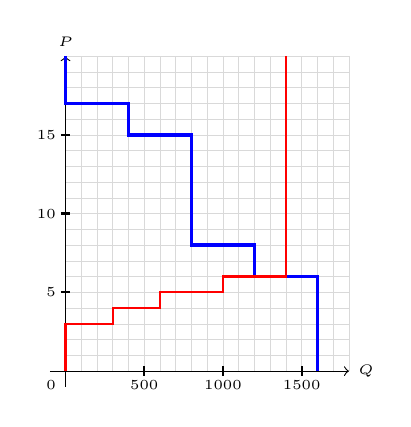
\begin{tikzpicture}[scale=.2]
            % create grid
            \draw[help lines, gray!30] (0,0) grid (18,20);
            
            % Draw axes
            \draw[->] (-1,0) -- (18,0) node[font=\tiny,right] {$Q$};
            \draw[->] (0,-1) -- (0,20) node[font=\tiny,above] {$P$};
          
            % Draw step functions
            \draw[blue, very thick] (0,20) -- (0,17) -- (4,17) -- (4,15) -- (8,15) -- (8,8) -- (12,8) -- (12,6) -- (16,6) -- (16,0);
            \draw[red, thick] (0,0) -- (0,3) -- (3,3) -- (3,4) -- (6,4) -- (6,5) -- (10,5) -- (10,6) -- (14,6) -- (14,20);
            
            % % Add labels
            \node[font=\tiny,below left] at (0,0) {$0$};
            \foreach \x in {5,10,15} {
              \node[font=\tiny,below] at (\x,0) {$\x00$};
            }
            \foreach \y in {5,10,15} {
              \node[font=\tiny,left] at (0,\y) {$\y$};
            }

            % % Add thicker ticks (Q)
            \draw[black, thick] (5,-0.3) -- (5,0.3);
            \draw[black, thick] (10,-0.3) -- (10,0.3);
            \draw[black, thick] (15,-0.3) -- (15,0.3);

            % % Add thicker ticks (P)
            \draw[black, thick] (-0.3,5) -- (0.3,5);
            \draw[black, thick] (-0.3,10) -- (0.3,10);
            \draw[black, thick] (-0.3,15) -- (0.3,15);
        \end{tikzpicture}
        \subcaption{\tiny Block 2 (T5-T8) \\ and Block 4 (T13-T16)}
    \end{subfigure}%
    \begin{subfigure}[c]{0.33\linewidth}
        \centering
        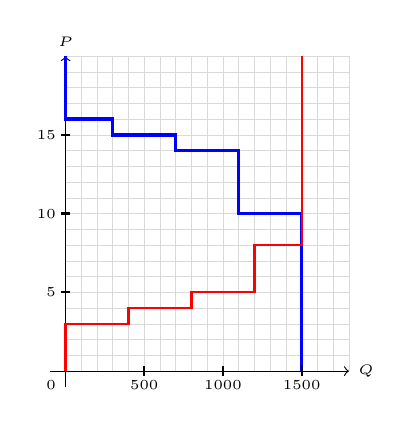
\begin{tikzpicture}[scale=.2]
            % create grid
            \draw[help lines, gray!30] (0,0) grid (18,20);
            
            % Draw axes
            \draw[->] (-1,0) -- (18,0) node[font=\tiny,right] {$Q$};
            \draw[->] (0,-1) -- (0,20) node[font=\tiny,above] {$P$};
          
            % Draw step functions
            \draw[blue, very thick] (0,20) -- (0,16) -- (3,16) -- (3,15) -- (7,15) -- (7,14) -- (11,14) -- (11,10) -- (15,10) -- (15,0);
            \draw[red, thick] (0,0) -- (0,3) -- (4,3) -- (4,4) -- (8,4) -- (8,5) -- (12,5) -- (12,8) -- (15,8) -- (15,20);
            
            % % Add labels
            \node[font=\tiny,below left] at (0,0) {$0$};
            \foreach \x in {5,10,15} {
              \node[font=\tiny,below] at (\x,0) {$\x00$};
            }
            \foreach \y in {5,10,15} {
              \node[font=\tiny,left] at (0,\y) {$\y$};
            }

            % % Add thicker ticks (Q)
            \draw[black, thick] (5,-0.3) -- (5,0.3);
            \draw[black, thick] (10,-0.3) -- (10,0.3);
            \draw[black, thick] (15,-0.3) -- (15,0.3);

            % % Add thicker ticks (P)
            \draw[black, thick] (-0.3,5) -- (0.3,5);
            \draw[black, thick] (-0.3,10) -- (0.3,10);
            \draw[black, thick] (-0.3,15) -- (0.3,15);
        \end{tikzpicture}
        \subcaption{\tiny Block 3 (T9 - T12)}
    \end{subfigure}
    \caption{\textbf{Contract configurations across trading blocks.}  \footnotesize
Vertical axis is price (ECU per share) and horizontal axis is quantity (shares). Each panel plots the step‐function demand schedule (thick blue) and supply schedule (red).  
The intersection of the two schedules determines the competitive‐equilibrium price–quantity pair for that block.  
Panel (a) applies to Blocks 1 (T1–T4) and 5 (T17–T20) of experiment; panel (b) to Blocks 2 (T5–T8) and 4 (T13–T16); panel (c) to Block 3 (T9–T12). }
% \label{fig:contract-configs}
    \label{fig:3contract_configs_new}
\end{figure}

\end{frame}


\begin{frame}{Experiment Design: Interface - CDA}
    \begin{figure}[H]
        \centering
        
\includegraphics[width=\textwidth]{figures/cda_ui.png}
        \caption{CDA UI}
        \label{fig:cda_ui}
    \end{figure}
\end{frame}

\begin{frame}{Experiment Design: Interface - CDA Animation}
  \animategraphics[loop,controls,width=\linewidth]{10}{figures/cda_animation/cda_animation-}{0}{252}
\end{frame}



\begin{frame}{Experiment Design: Interface - FLOW Animation}
  \animategraphics[loop,controls,width=\linewidth]{10}{figures/flow_animation/flow_animation-}{0}{419}
\end{frame}


\begin{frame}{Experiment Design: Interface - FLOW}
    \begin{figure}[H]
        \centering
        
\includegraphics[width=\textwidth]{figures/flow_ui.png}
        \caption{FLOW UI}
        \label{fig:flow_ui}
    \end{figure}
\end{frame}




\begin{frame}{Hypotheses}
    \begin{itemize}
        \item[H1] \textit{Traders will fragment orders more
(i.e., submit a larger number of smaller quantity orders) in CDA format than in Flow format.} %\pause
\vspace{0.3cm}
        \item[H2] \textit{Price volatility will be lower with the Flow format than with the CDA.}%\pause
\vspace{0.3cm}        
        \item[H3] \textit{(a) Trading volume with CDA and Flow formats will be similar. \\ (b) Both will move within each trading block towards the minimum volume that sustains competitive equilibrium.} %\pause
\vspace{0.3cm}        
        \item[H4] \textit{The CDA and Flow formats will exhibit similar levels of (a) informational and (b) allocative efficiency.} %\pause
    \end{itemize}
\end{frame}


\section{Results}

\begin{frame}{Summary of Results}

\begin{enumerate}
    \item[R1:] \textbf{Flow} Market format exhibits \textbf{fewer and larger orders}.  \pause 
    \vspace{0.5cm}
    
    \item[R2:] \textbf{Flow} format exhibits \textbf{lower price volatility} compared to the CDA.  \pause 
    \vspace{0.5cm}
    
    \item[R3:] Traded \textbf{Volume is lower in the Flow} Market than in the CDA.  \pause 
    \vspace{0.5cm}
    
    \item[R4:] Flow and CDA markets have \textbf{comparable} informational and allocative \textbf{efficiency}.  \pause 
    
\end{enumerate}



\end{frame}


\begin{frame}{Descriptive Stats: Traders' Behavior}
\begin{table}[H]
    \centering
    % \caption{Summary Statistics: Traders' Behavior}
    \resizebox{.95\textwidth}{!}{
    \begin{tabular}{lcccccc}
    \toprule
    ~                               & \multicolumn{2}{c}{T1 - T20} & \multicolumn{2}{c}{T1 - T10}  & \multicolumn{2}{c}{T11 - T20} \\
                                    & CDA       & FLOW      & CDA       & FLOW      & CDA       & FLOW      \\
    \midrule ↩
    % \multicolumn{7}{l}{\textbf{(a) Trader Behavior}} \\
    % \hline \\[-1.8ex]
     Number of Orders                       & 32       & 24            & 31       & 25            & 32        & 23            \\
     \hspace{3mm}Seller             & 17       & 12            & 17       & 13            & 17        & 11            \\
     \hspace{3mm}Buyer              & 15       & 12            & 15       & 12            & 15        & 12            \\
     % Order Size                     & 42       & 72            & 44       & 63            & 40        & 80            \\
     \\
     Quant. per Order                 & 113      & 182           & 115      & 180           & 111       & 185           \\
     \hspace{3mm}Seller             & 115      & 185           & 118      & 184           & 111       & 185           \\
     \hspace{3mm}Buyer              & 114      & 188           & 116      & 184           & 113       & 191           \\
     \\
     Order Price                    & 8.93     & [6.78, 12.64] & 9.18     & [7.15, 13.01] & 8.68      & [6.41, 12.28] \\
     \hspace{3mm}Seller             & 10.7     & [9.21, 15.46] & 11.13    & [9.76, 16.04] & 10.27     & [8.66, 14.88] \\
     \hspace{3mm}Buyer              & 6.9      & [4.22, 9.71]  & 7.01     & [4.26, 9.71]  & 6.79      & [4.19, 9.71]  \\

    \\
     Order Max Rate                 &           & 19.62         &           & 17.78         &           & 21.46         \\
     \hspace{3mm}Seller             &           & 19.67         &           & 18.06         &           & 21.29         \\
     \hspace{3mm}Buyer              &           & 20.15         &           & 17.93         &           & 22.37         \\
    \bottomrule
    \end{tabular}}
    \label{tab:summary_stat_trader}
\end{table}

\end{frame}

\begin{frame}{Descriptive Stats: Market Performance}
    
    \begin{table}
    \centering
    % \caption{Summary Statistics: Market Performance}
    % \renewcommand{\arraystretch}{1.1}
     \resizebox{\textheight}{!}{
    \begin{threeparttable}
    \begin{tabular}{lcccccc}
    \toprule
    
    ~                               & \multicolumn{2}{c}{T1 - T20} & \multicolumn{2}{c}{T1 - T10}  & \multicolumn{2}{c}{T11 - T20} \\
                                    & CDA       & FLOW      & CDA       & FLOW      & CDA       & FLOW      \\
    \midrule 
     \\[-1.8ex] 
      \multicolumn{7}{l}{\textit{\textbf{(a)} Price Statistics} (Avg. Equil Price = $9.8$ ECUs)} \\
    % \hline 
     \\[-1.8ex]    
     Clearing Prices ($P_t$, ECUs)              & 8.62      & 9.37      & 9.04      & 9.57      & 8.21      & 9.18      \\
     \hspace{3mm}(Std. Dev.)                    & (2.77)    & (2.54)    & (2.95)    & (2.75)    & (2.51)    & (2.29)    \\
     $ \lvert  P_{t}-P_{t - 1} \rvert $         & 0.57      & 0.39      & 0.58      & 0.39      & 0.55      & 0.4       \\
     Std. Dev. of $(\ln P_{t} - \ln P_{t - 1})$ & 0.14      & 0.07      & 0.15      & 0.07      & 0.13      & 0.07     \\    
     \\ [-1.8ex]
     \multicolumn{7}{l}{\textit{\textbf{(b)} Volume, Transaction Intensity}} \\
     \\ [-1.8ex]
     Traded Volume (shares)                     & 1138      & 959       & 1097      & 872       & 1179      & 1046      \\
     Traded Vol. / $Q_{\text{CE}}$. (\%)        & 93.6      & 78.8      & 90.3      & 71.1      & 96.9      & 86.4      \\
     Filled Contract / $Q_{\text{CE}}$ (\%)     & 85.2      & 77.1      & 81.0      & 69.8      & 89.3      & 84.5      \\
     Num. of Trans.                             & 14        &           & 13        &           & 15        &           \\
     Mean Transaction Size                      & 78        &           & 82        &           & 74        &           \\
     \hspace{3mm}(Std. Dev.)             & (61)      &           & (61)      &           & (60)      &           \\
     Clearing Rate ($q/sec$)                 &           & 9.37      &           & 9.54      &           & 9.2       \\
     \hspace{3mm}(Std. Dev.)             &           & (2.6)     &           & (2.8)     &           & (2.4)     \\
     \\ [-1.8ex]
     \multicolumn{7}{l}{\textit{\textbf{(c)} Efficiency and Buyer-Seller Inequality}} \\
     \\ [-1.8ex]
     Info. Effic.: $\lvert P_t - P_{\text{CE}} \rvert $        & 2.16      & 2.08      & 2.19      & 2.32      & 2.14      & 1.84      \\     
     Alloc. Effic.: $\Pi$ / $\Pi_{\text{CE}}$ ($\times 100$)          & 84.3      & 81.81     & 79.76     & 77.31     & 88.85     & 86.31     \\
     
     ${\Pi^{\text{buy}}}/{\Pi^{\text{buy}}_{\text{CE}}} - {\Pi^{\text{sell}}}/{\Pi^{\text{sell}}_{\text{CE}}}$ 
     ($\times 100$) & 53.7      & 11.18     & 27.38     & -5.16     & 80.03     & 27.51     \\
     \\[-1.8ex] 
    \bottomrule 
    \end{tabular}
    \begin{tablenotes}[para,flushleft]
      \footnotesize
    \end{tablenotes}
    \end{threeparttable}
   }
    \label{tab:summary_stat}
\end{table}
\end{frame}


\begin{frame}{Descriptive: Transaction Price Dynamics}
    \begin{figure}[H]
        \centering
        \begin{subfigure}[b]{0.85\textwidth}
            \centering
            
\includegraphics[width=1.15\linewidth]{figures/Grp-CDA-priceTrim.pdf}
            %\caption{CDA}
            \label{price_flow}
        \end{subfigure}
        \begin{subfigure}[b]{0.85\textwidth}
            \centering
            
\includegraphics[width=1.15\linewidth]{figures/Grp-Flow-priceTrim.pdf}
           % \caption{FLOW}
            \label{price_cda}
        \end{subfigure}
       % \caption{Clearing Prices}
    \end{figure}
    % \vspace{-15pt}
    % \scriptsize{The vertical dotted lines are period breaks. The first 10 seconds from each trading period are left out. The lighter colors represent individual groups.} 
\end{frame}

\begin{frame}{Descriptive: Volume and Surplus Dynamics}
    \begin{figure}
        \centering
        % First row: Volume Trends
        \begin{subfigure}[b]{0.48\linewidth}
            \centering
            
\includegraphics[width=\linewidth]{figures/groups_cda_quantity.png}
            \caption{CDA - Traded Volume}
            \label{fig:combined_volume_cda}
        \end{subfigure}%
        \hfill % Space between the figures
        \begin{subfigure}[b]{0.48\linewidth}
            \centering
            
\includegraphics[width=\linewidth]{figures/groups_flow_quantity.png}
            \caption{FLOW - Traded Volume}
            \label{fig:combined_volume_flow}
        \end{subfigure}
        
        % Second row: Realized Surplus
        \begin{subfigure}[b]{0.48\linewidth}
            \centering
            
\includegraphics[width=\linewidth]{figures/groups_cda_surplus.png}
            \caption{CDA - Realized Surplus}
            \label{fig:combined_surplus_cda}
        \end{subfigure}%
        \hfill % Space between the figures
        \begin{subfigure}[b]{0.48\linewidth}
            \centering
            
\includegraphics[width=\linewidth]{figures/groups_flow_surplus.png}
            \caption{FLOW - Realized Surplus}
            \label{fig:combined_surplus_flow}
        \end{subfigure}
    \end{figure}
\end{frame}



%%%%%%%%%%%%%%%%%%%%%%%%%%%%%%%%%%%%%%%%%%%%%%%%%%%%%%%%%%%%%%%%%%%%%%%%%%%%%%%%%%%%%


\section{Conclusions}

\begin{frame}{Conclusions}
\begin{itemize}
\item \textbf{First test} of Flow market format, comparing it to CDA in an induced-value setting BUT with finely divisible units. %\pause
% \item Traders' behavior and market performance (prices, quantities, and efficiency). 
\vspace{0.3cm}
\item Flow started worse than CDA but improved faster (learning).
\item Price \textbf{volatility} is lower in Flow.  %\pause
\item Some relative \textbf{undertrading} in Flow, but efficiency is comparable.
\item \textbf{Informational efficiency} |$P-P_{CE}$| was comparable. %\pause
\item Similar performance in \textbf{allocative efficiency}. %\pause
\item Buyer-seller asymmetry in Flow seems reduced.%\pause
\end{itemize} 
\vspace{0.4cm}

\begin{center}
{\large A first draft is available for those interested. \\ Suggestions are very welcome!}

\url{kristian@ucsc.edu}
    
\end{center}


\end{frame}







%%%%%%%%%%%%%%%%%%%%%%%%%%%%%%%%%%%%%%%%%%%%%%%%%%%%%%%%%%%%%%%%%%%%%%%%%%%%%%%%%%%%%

\section{Appendix}


\begin{frame}{Continuous Double Auction (CDA) Format}
processes standard limit orders.
\begin{itemize}
    \item These orders are defined by \textbf{three parameters}:$\rightarrow$ ``\underline{Buy/sell} up to \underline{$Q_{max}$} (shares) at a price of \underline{$P$} (dollars per share) or better."
\item Asynchronous order submission within a known time interval. 
\begin{itemize}
\item If a new order does not \textbf{cross} a queued contra-side order, then it is queued in the book. 
\item If it does cross, then it transacts immediately at the best price(s) on the other side of the market.
\end{itemize}
\item Strict \textbf{(price, time) priority}. If there is a tie on price, then older orders are filled first.
    \end{itemize} 
\end{frame}



\begin{frame}{CDA Timing Issues}
1. Early bird special  
    \begin{itemize}
        \item Since market supply and demand are discontinuous step functions of price, there is \textbf{no guarantee of a single point of intersection}: there can be excess of demand (supply), and often there is. 
        \item Hence, \textbf{an allocation rule} to determine $\alpha(t_0, t)$ is needed (e.g., time priority, or pro-rata)
\item In most existing financial markets, orders are \textbf{prioritized} based on \textbf{the time they arrive}, so high speed is rewarded
\item If an agent can \textbf{react to a relevant signal} (even if public) \textbf{faster} (even if only a tiny bit) than other traders, then she can \textbf{pick off stale orders} from other traders and reverse position after the information has spread in the market.
\item  Thus: tilted playing field, rent-seeking, toxic takers $\implies$ illiquidity, increased flash crash risk.
    \end{itemize}
    2. To avoid adverse price pressure, traders will want to \textbf{shred} large orders.
    \end{frame}


\subsection{Experiment Implementation}

\begin{frame}{Procedures}
    \begin{itemize}
        \item We paid the cumulative profits of all 20 payment periods
        \item Exchange rate is 1000 ECUs = 1 USD and show-up fee is 7 USD %\pause
        \item Experiment software was designed and developed at UCSC's LEEPS Laboratory
        \item Experiment sessions were conducted in person at LEEPS Laboratory
        \item So far have 5  FLOW and 5 CDA sessions
    \end{itemize}
\end{frame}

\subsection{Outcomes and Hypotheses}


\begin{frame}{Outcomes}
    \begin{itemize}
        \item For \textbf{trading behavior}, we study: 
     the number of orders, the size of the orders, submitted prices, and
     the maximum execution rate in Flow market. %\pause
        \item For \textbf{market performance}, we study:
        \begin{itemize}
        \item \textit{Absolute Price Change}, $|P_t - P_{t-1}|$. 
        \item \textit{Price volatility}, $(\ln P_t - \ln P_{t-1})$ 
         \item \textit{Trading Volume}, $Q$ (at the market-period level)
\item\textit{Informational [in]Efficiency},  \( |P_t - P_{\text{CE}}| \). 
    \item\textit{Allocative Efficiency}, measured as \( \Pi/\Pi_{\text{CE}}\) (at the market-period level). 
        \end{itemize}
     
    \end{itemize}
\end{frame}




\subsection{Regression Analysis}



\begin{frame}{Regression Analysis}
For each metric, we estimate: 
\begin{equation} \label{eq:reg}
    y_{g,t} = \alpha + \sum^{4}_{i = 1} \left(\beta_i \; \text{Block}_i\right) + \gamma \; \text{FLOW}_{g,t} + \theta \; \text{Period}_{g,t} + \epsilon_{g,t}
\end{equation}
where $y_{g,t}$ is an outcome  indexed by group (i.e., session) and time, and the $\gamma$ for the dummy variable $\text{FLOW}_{g,t}$ is the treatment effect. %\pause

We control for: 
\begin{itemize}
\item S-D configuration, via  block fixed effect coefficients $\beta_i$,  
\item time trends, via coefficient $\theta$ for period number $\text{Period}_{g,t}$, and
\item session effects, via clustered s.e.'s.
\end{itemize} %\pause
 
% Dependent variables $y$ here are: deviations from CE $ =\mid P^W_t - P_{CE}\mid$, 
% mean absolute interval-to-interval price change $=\mid P^W_{t} - P^W_{t - 1}\mid$, and 
% volatility $=Std\left(\ln P^W_{t} - \ln P^W_{t - 1}\right).$
\end{frame}



%%%%%%%%%%%%%%%%%%%%%%
\begin{frame}{H1: Regressions for Number and size of orders}
\begin{table}[H]
\centering    
\caption{Regression: Traders' Behavior}
\resizebox{\textheight}{!}{
\begin{threeparttable}
\begin{tabular}{@{\extracolsep{5pt}}lcccc}
\toprule
& \multicolumn{2}{c}{Number of Orders} & \multicolumn{2}{c}{Order Size} \\
% & \cline{1-4}
\cmidrule{2-5}
& T1-T20 & T11-T20 & T1-T20 & T11-T20 \\
& (1) & (2) & (3) & (4) \\
\midrule
Intercept & 36.170$^{***}$ & 41.770$^{***}$ & 29.481$^{*}$ & 15.523$^{}$ \\
 & (4.702) & (6.710) & (15.726) & (23.527) \\
Flow Format (=1) & -7.840$^{***}$ & -8.820$^{***}$ & 10.314$^{*}$ & 17.437$^{***}$ \\
 & (1.512) & (0.827) & (5.319) & (4.700) \\
Period Number & -0.300$^{}$ & -0.576$^{*}$ & 2.384$^{***}$ & 2.946$^{**}$ \\
 & (0.219) & (0.347) & (0.805) & (1.296) \\
\midrule
Observations & 200 & 100 & 200 & 100 \\
Adjusted $R^2$ & 0.406 & 0.567 & 0.240 & 0.283 \\
\midrule
CDA avg. & 32 & 32 & 42 & 40 \\
\bottomrule
\end{tabular}
\begin{tablenotes}[para,flushleft]
\footnotesize
\textit{Note:} $^{*}$p$<$0.1; $^{**}$p$<$0.05; $^{***}$p$<$0.01. The standard errors within parentheses are cluster-robust at the group level. We omit the coefficients of the block dummies. 
\end{tablenotes}
\end{threeparttable}
}
\label{tab:TradersBehavior}
\end{table}
\end{frame}


\begin{frame}{Result 1: Flow Market format exhibits fewer and larger orders than CDA}
\begin{itemize}
\item Flow market format has 8-9 fewer orders submitted per period than the 32 in CDA ($p < 0.01$).
\item But the orders are larger, especially in later periods (by $\sim 17$, compared to $\sim$40 in CDA, ($p < 0.01$).  
\item Taken together, these results suggest that the Flow market format shreds orders more effectively than the CDA. 
% \item Overall lower trading volume in Flow, by $\sim$ 130 shares in later periods ($p < 0.05$).
\item Order size trends significantly upward over time.
\end{itemize}   
\end{frame}



%%%%%%%%%%%%%%%%%%%%%%%%

\begin{frame}{H2: Price Volatility Regression}

\begin{table}[H]
\centering    
\caption{Regression: Price Volatility}
\resizebox{\textheight}{!}{
\begin{threeparttable}
\begin{tabular}{@{\extracolsep{5pt}}lcccc}
\toprule
& \multicolumn{2}{c}{$\lvert P_{t} - P_{t - 1}\rvert$} & \multicolumn{2}{c}{SD$\left(\ln P_{t} - \ln P_{t - 1}\right)$} \\
\cmidrule{2-5}
& T1-T20 & T11-T20 & T1-T20 & T11-T20 \\
& (1) & (2) & (3) & (4) \\
\midrule
Intercept & 2.456$^{***}$ & 2.924$^{***}$ & 0.345$^{***}$ & 0.391$^{***}$ \\
 & (0.462) & (0.905) & (0.069) & (0.124) \\
Flow Format (=1) & -0.736$^{***}$ & -0.552$^{***}$ & -0.070$^{***}$ & -0.061$^{***}$ \\
 & (0.119) & (0.146) & (0.016) & (0.023) \\
Period number & -0.062$^{***}$ & -0.094$^{**}$ & -0.010$^{***}$ & -0.013$^{*}$ \\
 & (0.024) & (0.044) & (0.004) & (0.007) \\
\midrule
Observations & 4,600 & 2,300 & 200 & 100 \\
Adjusted $R^2$ & 0.139 & 0.118 & 0.307 & 0.282 \\
\midrule
CDA avg. & 0.57 & 0.55 & 0.14 & 0.13 \\
\bottomrule
\end{tabular}
\begin{tablenotes}[para,flushleft]
\footnotesize
\textit{Note:} $^{*}$p$<$0.1; $^{**}$p$<$0.05; $^{***}$p$<$0.01. The standard errors within parentheses are cluster-robust at the group level. We omit the coefficients of the block dummies. 
\end{tablenotes}
\end{threeparttable}
}
\label{tab:PriceVolatility}
\end{table}

\end{frame}



\begin{frame}{Result 2: Flow format exhibits lower price volatility compared to the CDA}
\begin{itemize}
% \item \textbf{Price efficiency} is similar (insignificantly lower in Flow).
\item Significantly \textbf{smaller price changes} (by $\sim 0.7$, $p<0.01$) in Flow, 
\item Also, significantly lower \textbf{volatility} (by $\sim$7 pp, about half!, $p<0.01$).
\item Significant \textbf{improvement over time} in these metrics in both formats.
(Weak evidence elsewhere for more rapid improvement with Flow). 
\end{itemize}   
\end{frame}



%%%%%%%%%%%%%%%%%

\begin{frame}{H3: Traded Volume Regression}

\begin{table}
\centering    
\caption{Regression: Traded Volume}
\resizebox{\textheight}{!}{
\begin{threeparttable}
\begin{tabular}{@{\extracolsep{5pt}}lcccc}
\toprule
& \multicolumn{2}{c}{Traded Volume} & \multicolumn{2}{c}{Filled Cont. Q / $Q_{CE}$} \\
\cmidrule{2-5}
& T1-T20 & T11-T20 & T1-T20 & T11-T20 \\
& (1) & (2) & (3) & (4) \\
\midrule
Intercept & 746.583$^{***}$ & 728.025$^{***}$ & 0.634$^{***}$ & 0.641$^{***}$ \\
 & (116.483) & (134.216) & (0.117) & (0.122) \\
Flow Format (=1) & -178.764$^{***}$ & -132.314$^{**}$ & -0.080$^{*}$ & -0.048$^{}$ \\
 & (34.432) & (63.499) & (0.044) & (0.034) \\
Period number & 18.866$^{***}$ & 18.613$^{**}$ & 0.016$^{***}$ & 0.014$^{**}$ \\
 & (6.030) & (7.868) & (0.005) & (0.006) \\
\midrule
Observations & 200 & 100 & 200 & 100 \\
Adjusted $R^2$ & 0.454 & 0.322 & 0.264 & 0.150 \\
\midrule
CDA avg. & 1138 & 1179 & 85.2 & 89.3 \\
\bottomrule
\end{tabular}
\begin{tablenotes}[para]
\footnotesize
\textit{Note:} $^{*}$p$<$0.1; $^{**}$p$<$0.05; $^{***}$p$<$0.01. The standard errors within parentheses are cluster-robust at the group level. We omit the coefficients of the block dummies. 
\end{tablenotes}
\end{threeparttable}
}
\label{tab:Volume}
\end{table}

\end{frame}

\begin{frame}{Result 3: Traded Volume is lower in the Flow Market than in the CDA.}
\begin{itemize}
% \item Flow market format has 8-9 fewer orders submitted per period than the 32 in CDA ($p < 0.01$).
% \item But the orders are larger, especially in later periods (by $\sim 17$, compared to $\sim$40 in CDA, $p < 0.01$).  
% \item Taken together, these results suggest that the Flow market format shreds orders more effectively than the CDA. 
\item Overall lower trading volume in Flow, by $\sim$ 130 shares in later periods ($p < 0.05$).
\item Volume in Flow trends significantly upward over time.
\item The significantly lower trading volume in Flow format does not greatly impair filling contracts; the treatment effect is insignificant.
\end{itemize}   
\end{frame}





%%%%%%%%%%%%%%%%%%%




\begin{frame}{H4: Informational and Allocative Efficiency Regression}

\begin{table}
\centering    
\caption{Regression: Efficiency and Buyer-Seller Disparity}
\resizebox{\textheight}{!}{
\begin{threeparttable}
\begin{tabular}{@{\extracolsep{5pt}}lcccccc}
\toprule
& \multicolumn{2}{c}{$\lvert P_t - P_{\text{CE}}\rvert$} & \multicolumn{2}{c}{Realized Surplus (\%)} & \multicolumn{2}{c}{Buyer-Seller Disparity} \\
\cmidrule{2-7}
& T1-T20 & T11-T20 & T1-T20 & T11-T20 & T1-T20 & T11-T20 \\
& (1) & (2) & (3) & (4) & (5) & (6) \\
\midrule
Intercept & 7.813$^{***}$ & 7.970$^{***}$ & 0.521$^{***}$ & 0.627$^{***}$ & 10327$^{***}$ & 14453$^{***}$ \\
 & (0.840) & (0.997) & (0.109) & (0.138) & (1809) & (2834) \\
Flow Format (=1) & -0.116$^{}$ & -0.191$^{}$ & -0.025$^{}$ & -0.025$^{}$ & -1608$^{}$ & -2082$^{*}$ \\
 & (0.218) & (0.328) & (0.035) & (0.030) & (1113) & (1072) \\
Period number & -0.228$^{***}$ & -0.234$^{***}$ & 0.020$^{***}$ & 0.014$^{**}$ & -92$^{}$ & -302$^{*}$ \\
 & (0.052) & (0.065) & (0.005) & (0.007) & (107) & (174) \\
\midrule
Observations & 4,800 & 2,400 & 200 & 100 & 200 & 100 \\
Adjusted $R^2$ & 0.317 & 0.446 & 0.291 & 0.052 & 0.779 & 0.805 \\
\midrule
CDA avg. & 2.16 & 2.14 & 84.3 & 88.85 & 2537 & 3417 \\
\bottomrule
\end{tabular}
\begin{tablenotes}[para]
\footnotesize
\textit{Note:} $^{*}$p$<$0.1; $^{**}$p$<$0.05; $^{***}$p$<$0.01. The standard errors within parentheses are cluster-robust at the group level. Buyer-Seller Disparity is defined as $({\Pi^{\text{buy}}}-{\Pi^{\text{buy}}_{\text{CE}}})-({\Pi^{\text{sell}}}-{\Pi^{\text{sell}}_{\text{CE}}})$. We omit the coefficients of the block dummies. 
\end{tablenotes}
\end{threeparttable}
}
\label{tab:EfficiencyAndDisparity}
\end{table}
\end{frame}


\begin{frame}{Result 4: Flow and CDA markets have comparable in informational and allocative efficiency}
\begin{itemize}
\item Both informational and allocative efficiency comparisons yield insignificant differences between the two formats.  

\item Informational (in)efficiency is similar. The price deviation from $P_{CE}$ is lower in Flow, but the difference is statistically insignificant.

\item Allocative efficiency is 2.5\% lower in Flow but also statistically insignificant. %\pause
\vspace{1cm}
\item (\textbf{Additional Result}) The Flow profit advantage (relative to CE) of buyers over sellers is less than half of that for CDA by the second half of periods but so noisy that the treatment effect is significant only at 10\% level. 
\end{itemize}   

\end{frame}


\begin{frame}{Disparity in Buyer-Seller Profits}
    \begin{figure}[H] 
        \centering
        \caption{Profit / CE Profits - Distribution}
        \begin{subfigure}[b]{.5\linewidth}
            \centering
            \begin{adjustbox}{trim=0 0 0 {.11\height}, clip=true}
                
\includegraphics[width=\linewidth]{figures/group_gross_profits_cdf.png}
            \end{adjustbox}
            \subcaption{\tiny T1-T20}
        \end{subfigure}%
        \begin{subfigure}[b]{.5\linewidth}
            \centering
            \begin{adjustbox}{trim=0 0 0 {.11\height}, clip=true}
                
\includegraphics[width=\linewidth]{figures/group_gross_profits_last_cdf.png}
            \end{adjustbox}
            \subcaption{\tiny T11-T20}
        \end{subfigure}
        \label{fig:norm_profits}
    \end{figure}
    
\end{frame}






    
\end{document}


